%% ************************************************
%% Universidade Nova de Lisboa
%% NOVA Information Management School
%% Computação em Estatística e Gestão de Informação
%% Júlio Caineta, 2015
%% ************************************************
\documentclass{exam}
\usepackage[utf8]{inputenc}
\usepackage{amsmath}
\usepackage[portuguese]{babel}
\usepackage[hidelinks,pdfusetitle]{hyperref}
\author{Júlio Caineta}
\title{CEGI 2014/2015 - Exercícios 3}
\usepackage{lastpage}
\usepackage{minted}
\usepackage{gensymb}
\usepackage{wrapfig}
\usepackage{tabulary}
\usepackage{graphicx}
%\usepackage{color}
\cfoot{Página \thepage\ de \pageref{LastPage}}
\renewcommand{\solutiontitle}{\noindent\textbf{Solução:}\par\noindent}
\newminted{r}{autogobble}
\newmintinline{r}{}
 
\printanswers
%\shadedsolutions

\begin{document}
 
\begin{center}
\textsc {\small NOVA IMS -- Universidade Nova de Lisboa} \\
\textsc {Computação em Estatística e Gestão de Informação -- 2º Semestre 2014/15}
\vspace{5mm} \\
{\large Exercícios 3}
\end{center}
 
\vspace{5mm}

\section*{Funções}

Em \textbf{R}, as funções são também objectos e podem ser manipuladas como tal. Têm três principais propriedades:

\begin{description}
	\item[argumentos] Lista dos parâmetros que a função vai receber, em que alguns podem ter um valor por defeito e ser opcionais. Uma forma rápida de consultar os argumentos de uma função é através da função \mintinline{r}{args}.
	\item[corpo]  Ao conjunto de expressões avaliado na execução da função chama-se corpo da função. É possível visualizar o corpo de uma função através da função \mintinline{r}{body}.
	\item[ambiente] Uma função é definida num determinado ambiente (\textit{environment}) activo, o que irá determinar os objectos visíveis e acessíveis pela função.
\end{description}

\begin{questions}
	\question Crie uma função que faça a conversão de graus Fahrenheit (\degree F) para graus Celsius (\degree C) , sabendo que a sua relação é dada pela \autoref{ftoc}.
	
	\begin{equation}
	\label{ftoc}
		\degree C = (\degree F - 32) \div 1,8	
	\end{equation}
	
	Teste a sua função para saber quantos graus Celsius correspondem a 159,3 \degree F, uma das temperaturas registadas mais altas de sempre na superfície da Terra, no deserto de Lut, no Irão.
	
	\begin{solution}
		\begin{rcode}
			f2c = function(fhr) {
				cls = (fhr - 32) / 1.8
				return(cls)
			}
			
			> f2c(159.3)
			[1] 70.72222
		\end{rcode}
	\end{solution}
	
	\question Expanda a sua função para, opcionalmente, também fazer a conversão de graus Celsius para Fahrenheit. A relação inversa é dada pela \autoref{ctof}.
	
	\begin{equation}
	\label{ctof}
		\degree F = (\degree C \times 1.8) + 32
	\end{equation}
	
	\begin{solution}
		\begin{rcode}
			converte.temp = function(temp, to="C") {
				if (to == "C") {
					x = (temp - 32) / 1.8
				} else if (to == "F") {
					x = temp * 1.8 + 32
				} else {
					stop(cat("opção inválida: ", to, "\n"))
				}
				return(x)
			}
			
			> converte.temp(100)
			[1] 37.77778
			> converte.temp(100,"F")
			[1] 212
			> converte.temp(100,"A")
			opção inválida:  A 
			Error in converte.temp(100, "A") : 
		\end{rcode}
	\end{solution}
	
	\question Atente ao seguinte bloco de código:
		\begin{rcode}
			x = 2
			z = 56.3
			f = function(x) {
			      a = 34
			      y = x / 4 * a * z
			      y
			    }
			f(21)
			a
		\end{rcode}
	Qual o valor das variáveis \mintinline{R}{a}, \mintinline{R}{x} e \mintinline{R}{z} dentro do ambiente da função? O que aconteceu ao valor da variável \mintinline{R}{a} após a execução da função?
	
	\begin{solution}
		\begin{rcode}
			f = function(x) {
				a = 34
				y = x / 4 * a * z
				cat("Variável x: ", x, "\nVariável a: ", a, "\nVariável z: ", z, "\n")
				y
			}
			
			> x = 2
			> z = 56.3
			> f(21)
			Variável x:  21 
			Variável a:  34 
			Variável z:  56.3 
			[1] 10049.55
		\end{rcode}
		Os valores visualizados correspondem aos valores que aquelas variáveis têm \textbf{dentro} da função:
		\begin{itemize}
			\item A variável \rinline{x} toma o valor passado como argumento da função. Não é o mesmo objecto que existe fora da função, embora tenha o mesmo nome (existem em ambientes diferentes).
			\item A variável \rinline{a} só existe dentro da função e tem o valor que recebe dentro desta.
			\item A variável \rinline{z} existe fora da função, mas quando acedida dentro da função, como não existe nenhum outro objecto com o mesmo nome, é procurado um objecto com esse nome no ambiente imediatamente acima do ambiente da função \rinline{f}.
		\end{itemize}
	\end{solution}
	
	\question Escreva três funções que recebam um \mintinline{R}{data.frame} e devolvam, por cada coluna:
		\begin{itemize}
			\item o máximo;
			\item o mínimo;
			\item a média.
		\end{itemize}
	Escreva duas versões para cada caso: uma recorrendo a um ciclo; e outra sem recorrer (explicitamente) a ciclos. Defina ainda o argumento opcional \mintinline{R}{first.n}, onde o utilizador poderá escolher para encontrar os referidos valores apenas considerando os primeiros \textit{n} elementos de cada coluna. Teste as suas funções com o conjunto de dados \mintinline{R}{iris}.
	
	\begin{solution}
		Versões recorrendo a ciclos:
		\begin{rcode}
			# máximo, usando um ciclo while
			maximo = function(tabela) {
				coluna = 1
				maxs = c()
				while (coluna <= ncol(tabela)) {
					maxs = c(maxs, max(tabela[ , coluna]))
					coluna = coluna + 1
				}
				return(maxs)
			}
			# mínimo, usando um ciclo for
			minimo = function(tabela) {
				mins = vector()
				for (coluna in tabela) {
					mins = c(mins, min(coluna))
				}
				mins
			}
			# média, usando um ciclo repeat, começando na última coluna
			media = function(tabela) {
				meds = NULL
				cols = ncol(tabela)
				repeat {
					if (!cols) {
						break
					}
					meds = c(meds, mean(tabela[ , cols]))
					cols = cols - 1
				}
				return(meds)
			}
		\end{rcode}
		
		Versões segundo o paradigma de programação funcional:
		\begin{rcode}
			# máximo
			maximo = function(tabela) {
				apply(tabela, 2, max)
			}
			# mínimo
			minimo = function(tabela) {
				apply(tabela, 2, min)
			}
			# média
			media = function(tabela) {
				apply(tabela, 2, mean)
			}
		\end{rcode}
		
		Falta agora acrescentar a funcionalidade opcional em que o utilizador poderá escolher para considerar apenas os primeiros \textit{n} elementos de cada coluna. Segue-se um exemplo para a última função mostrada. A alteração das restantes funções poderá ser feita de forma análoga.
		
		\begin{rcode}
			# média com argumento opcional
			media = function(tabela, first.n=nrow(tabela)) {
				apply(tabela[1:first.n, ], 2, mean)
			}
		\end{rcode}
		
		Exemplo de aplicação com a tabela \rinline{iris}:
		\begin{rcode}
			> media(iris[, -5])
			Sepal.Length  Sepal.Width Petal.Length  Petal.Width 
			5.843333     3.057333     3.758000     1.199333 
			> media(iris[, -5], 10)
			Sepal.Length  Sepal.Width Petal.Length  Petal.Width 
			4.86         3.31         1.45         0.22 
		\end{rcode}
	\end{solution}
	
	\question Assuma que gosta de coleccionar flores de Iris (\autoref{fig:iris}). Dispõe de uma tabela onde anota algumas das propriedades destas flores, registando, para cada exemplar, o valor de cada uma destas propriedades: comprimento e largura da pétala; comprimento e largura da sépala. A \autoref{tab:iris} mostra um excerto dessa tabela.
	
	\begin{figure}[t]
	   	\vspace{-40pt}
		\centering
		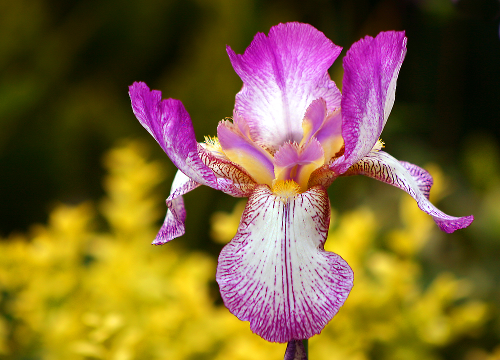
\includegraphics[width=0.4\linewidth]{Lilla_iris_randers}
		 \vspace{-10pt}
		\caption{\textit{Iris sibirica} (fonte: wikimedia.org).}
		\label{fig:iris}
	\end{figure}
	
%	\begin{wrapfigure}{!t}{0.5\linewidth}
%		\centering
%		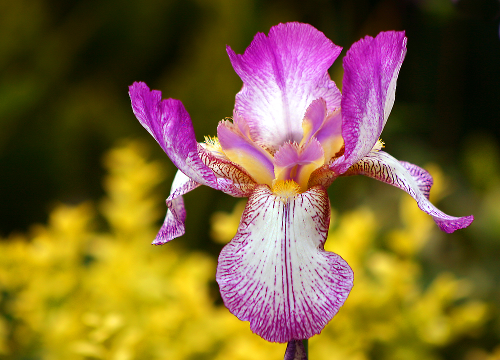
\includegraphics[width=0.4\linewidth]{Lilla_iris_randers}
%		\caption{Dummy figure.}
%		\label{fig:myfig}
%	\end{wrapfigure}

	\begin{table}[h]
		\begin{tabulary}{\textwidth}{|C|C|C|C|C|c|}
			\hline Número do examplar & Comprimento da Sépala & Largura da Sépala & Comprimento da Pétala & Largura da Pétala & Espécie \\ 
			\hline 1 & 5,1 & 3,5 & 1,4 & 0,2 & Setosa \\ 
			\hline 51 & 7,0 & 3,2 & 4,7 & 1,4 & Versicolor \\ 
			\hline 101 & 6,3 & 3,3 & 6,0 & 2,5 & Virginica \\ 
			\hline 
		\end{tabulary}
		\caption{Excerto da tabela com os registos das flores Iris, disponível em \textbf{R} na variável \mintinline{R}{iris}.}
		\label{tab:iris}
	\end{table}
	
	Após uma ida ao campo, uma nova amostra foi colhida. O novo exemplar tem as características indicadas na \autoref{tab:amostra}.
	
		\begin{table}[h]
			\begin{tabulary}{0.9\textwidth}{|C|C|C|C|C|}
				\hline Número do examplar & Comprimento da Sépala & Largura da Sépala & Comprimento da Pétala & Largura da Pétala \\ 
				\hline Nova amostra & 4,7 & 3,2 & 1,7 & 0,3 \\  
				\hline
			\end{tabulary}
			\caption{Características da nova amostra de flor Iris.}
			\label{tab:amostra}
		\end{table}
		
	O problema consiste em descobrir a que espécie pertence.
	
	Este é um problema típico de classificação\footnote{\url{https://en.wikipedia.org/wiki/Statistical_classification}}. Noutra disciplina, aprenderá mais sobre os métodos de classificação. Por agora, pode resolver este problema com uma implementação simples do algoritmo dos \textit{k}-vizinhos mais próximos\footnote{\url{https://en.wikipedia.org/wiki/K-nearest_neighbors_algorithm}}:
	
	\begin{itemize}
		\item Considere que cada característica tem o mesmo peso;
		\item Cada uma das características pode ser vista como um eixo (ou variável), então é como se tivesse quatro dimensões;
		\item A nova amostra será classificada como sendo da mesma espécie que o vizinho mais próximo ($k=1$) no conjunto de dados.
		\item Considere a distância como a distância Euclidiana\footnote{\url{https://en.wikipedia.org/wiki/Euclidean_distance}}.
	\end{itemize}
	
	Resolva este problema aplicando uma função sobre o \mintinline{R}{data.frame} \mintinline{R}{iris}.
	
	\begin{solution}
		Solução com uma linha de código:
		\begin{rcode}
			> iris$Species[which.min(apply(iris[, -5], 1,
			+ function(x) sum((x - c(4.7, 3.2, 1.7, 0.3))^2)))]
			[1] setosa
			Levels: setosa versicolor virginica
		\end{rcode}
		Agora em mais passos:
		\begin{rcode}
			amostra = c(4.7, 3.2, 1.7, 0.3)
			dist.euclidiana = function (vec1, vec2) {
				diff = vec1 - vec2
				square = diff^2
				return(sum(square))
			}
			distancias = apply(iris[, -5], 1, dist.euclidiana, vec2=amostra)
			indice_do_minimo = which.min(distancias)
			especie_amostra = iris$Species[indice_do_minimo]
			
			> especie_amostra
			[1] setosa
			Levels: setosa versicolor virginica
		\end{rcode}
		\textbf{Nota:} não é necessário calcular a Distância Euclidiana propriamente dita, basta calcular o seu quadrado -- a relação de ordem é preservada e o seu cálculo é menos exigente em termos computacionais. É por esse motivo que a função \rinline{sqrt} não foi usada nesta solução.
	\end{solution}
	
\end{questions}

\end{document}